\documentclass[tikz,border=12pt]{standalone}
\usepackage[T1]{fontenc}
\usepackage{mathpazo}
\usepackage{amsmath,amssymb}
\usetikzlibrary{arrows.meta, positioning, calc, decorations.pathreplacing, patterns}

\definecolor{stblue}{HTML}{7B97AD}
\definecolor{rwgold}{HTML}{B8995E}
\definecolor{sage}{HTML}{7A9A7E}
\definecolor{dkbrown}{HTML}{3D3530}
\definecolor{wmgray}{HTML}{7B7067}
\definecolor{cream}{HTML}{F9F6F0}
\definecolor{border}{HTML}{D4C9B8}
\definecolor{terracotta}{HTML}{C47A6A}
\definecolor{lavender}{HTML}{907EA0}

\begin{document}
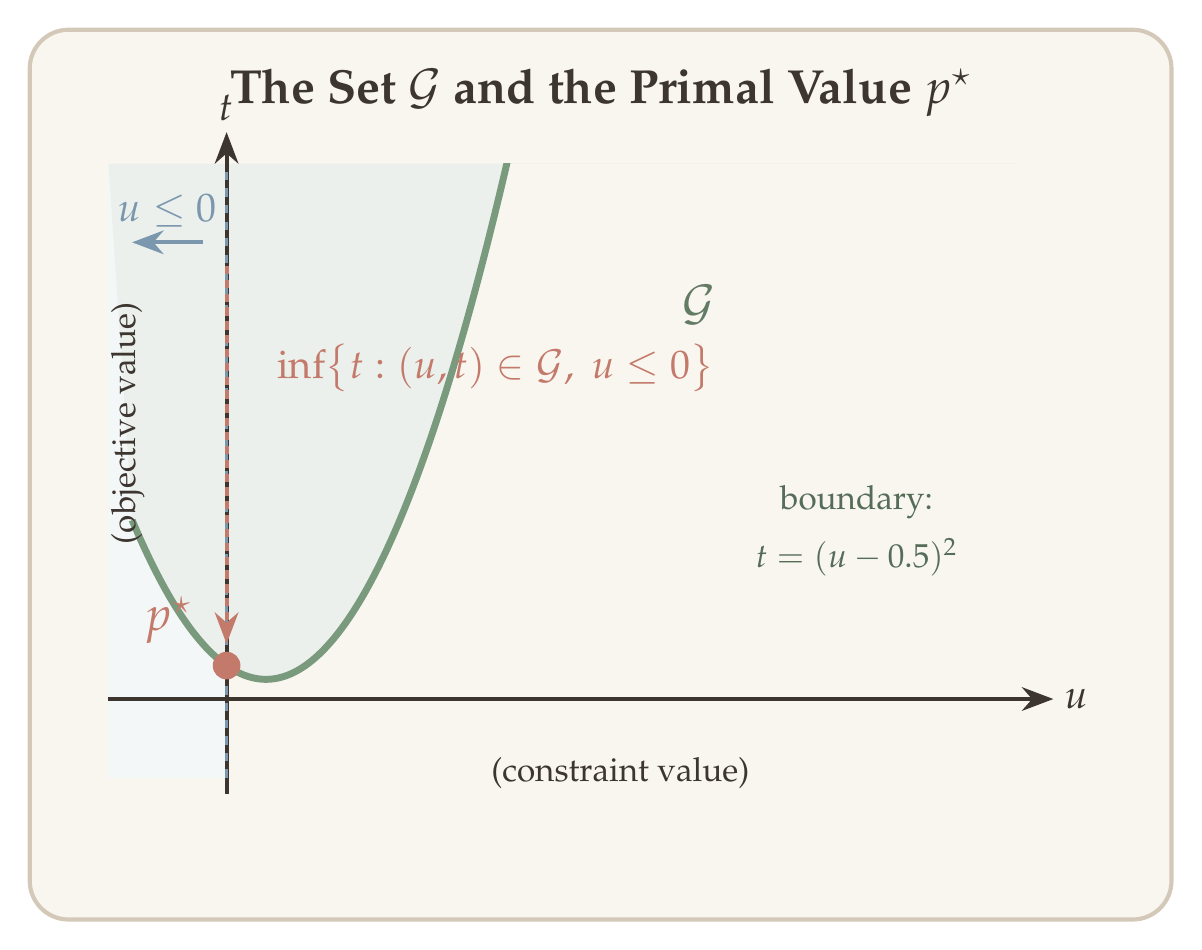
\begin{tikzpicture}[>={Stealth[length=4mm, width=3mm]}, line width=1.5pt]

% Background
\fill[cream, rounded corners=14pt] (-2.5,-2.8) rectangle (12,8.5);
\draw[border, line width=1.5pt, rounded corners=14pt] (-2.5,-2.8) rectangle (12,8.5);

% Title
\node[font=\LARGE\bfseries, text=dkbrown] at (4.75,7.7)
  {The Set $\mathcal{G}$ and the Primal Value $p^\star$};

% --- Fills and shapes (drawn BEFORE axes) ---

% Shading for u<=0 region
\fill[stblue!8] (-1.5,-1) rectangle (0,6.8);

% Fill the set G: parabola below, extends up
\begin{scope}
\clip (-1.5,-1) rectangle (10,6.8);
\fill[sage!15]
  plot[domain=-1.2:9, samples=80, smooth] ({(\x)}, {(\x-0.5)*(\x-0.5)*0.7 + 0.25})
  -- (10,6.8) -- (-1.5,6.8) -- cycle;
\draw[sage, line width=2.5pt]
  plot[domain=-1.2:5.5, samples=80, smooth] ({(\x)}, {(\x-0.5)*(\x-0.5)*0.7 + 0.25});
\end{scope}

% --- Axes (drawn AFTER fills so they remain visible) ---
\draw[->, dkbrown, line width=1.5pt] (-1.5,0) -- (10.5,0)
  node[right, font=\Large, text=dkbrown] {$u$};
\draw[->, dkbrown, line width=1.5pt] (0,-1.2) -- (0,7.2)
  node[above, font=\Large, text=dkbrown] {$t$};

% u<=0 dashed boundary (on top of axis)
\draw[stblue, line width=1pt, dashed] (0,-1) -- (0,6.8);

% --- Labels and annotations ---
\node[font=\large, text=dkbrown, below] at (5,-0.6) {(constraint value)};
\node[font=\large, text=dkbrown, rotate=90, above] at (-0.9,3.5) {(objective value)};
\node[font=\Large, text=stblue] at (-0.75,6.2) {$u \le 0$};

% Label for G
\node[font=\LARGE\bfseries, text=sage!80!black] at (6,5) {$\mathcal{G}$};

% Annotation for boundary
\node[font=\large, text=sage!70!black, align=center] at (8,2.5)
  {boundary:};
\node[font=\large, text=sage!70!black, align=center] at (8,1.8)
  {$t = (u - 0.5)^2$};

% Point p* at u=0
\fill[terracotta] (0,0.425) circle (5pt);
\node[font=\LARGE\bfseries, text=terracotta, left] at (-0.3,1.0) {$p^\star$};

% Downward arrow to show p* is the minimum t on G at u<=0
\draw[terracotta, line width=1.5pt, ->, densely dashed] (0,5.5) -- (0,0.7);
\node[font=\Large, text=terracotta, right, align=left] at (0.5,4.2)
  {$\inf\bigl\{t : (u,t) \in \mathcal{G},\; u \le 0\bigr\}$};

% Arrow showing u<=0 direction
\draw[stblue, line width=1.5pt, ->] (-0.3,5.8) -- (-1.2,5.8);

\end{tikzpicture}
\end{document}
